
In this section we talk about the context underlighing our contribution and present the motivations that lead to our approach.

\subsection{Context: Mobile Crowd-Sensing Platforms}

The crowd-sensing platforms have a large application domain.
Applications encompass application performance monitoring (\emph{e.g.}, OpenSignal\footnote{\url{http://opensignal.com}}), environment monitoring (air quality\footnote{\url{http://citizensensor.cc}}), etc.

Privacy-preserving in this context is a key challenge to address.
The platforms must balance to find an equilibrium between the level of the users' privacy-preserving and the quality of the data that are collected.
Indeed, if a crowd-sensing platform put a lot of consideration in the privacy preserving, the collected data could be degraded depending to the data type.
At last, if a crowd-sensing platform does not care about the privacy of its users, these last may not want to contribute to it.
To the best of our knowledge, privacy-preserving techniques are often deployed on the server side~\cite{DBLP:conf/mobisys/CorneliusKKPST08}~\cite{DBLP:conf/dais/HadererRS13}.
For instance, for the Geo-located data, there can be anonymized \emph{a posteriori}~\cite{DBLP:conf/icdcs/PrimaultMB15}.

The context to this proposal is based on the APISENSE crowd-sensing platform that provide an Android application to collect data from users that subscribe to data collect campaign and contribute with their mobile devices.
Because the platform apply privacy-preserving technics on the server side, it does not protect from malicious behaviors during the upload phase.
The data that come from a user are unmodified and are his own data.
This is the data that were produced by this specific user.
A user is therefore forced to trust the server that receives his data.

\subsection{Motivations: Data Dissemination Threats}

In the APISENSE platform, a collect server can be managed by an external organization.
The collect servers are called honneycomb.
The way of having a single trusted server that handle all users data sending is not practicable.
Having multiple server is a requirement in this kind of platform and we can say that no server can be trusted.

A key challenge in the crowd-sensing platforms is to avoid central trusted server that present a single point of failure that need to be address.

The current process of data collection is represented in the Figure~\ref{Threat} (the arrows represente the data flow).

\begin{figure*}[h]
    \centering
    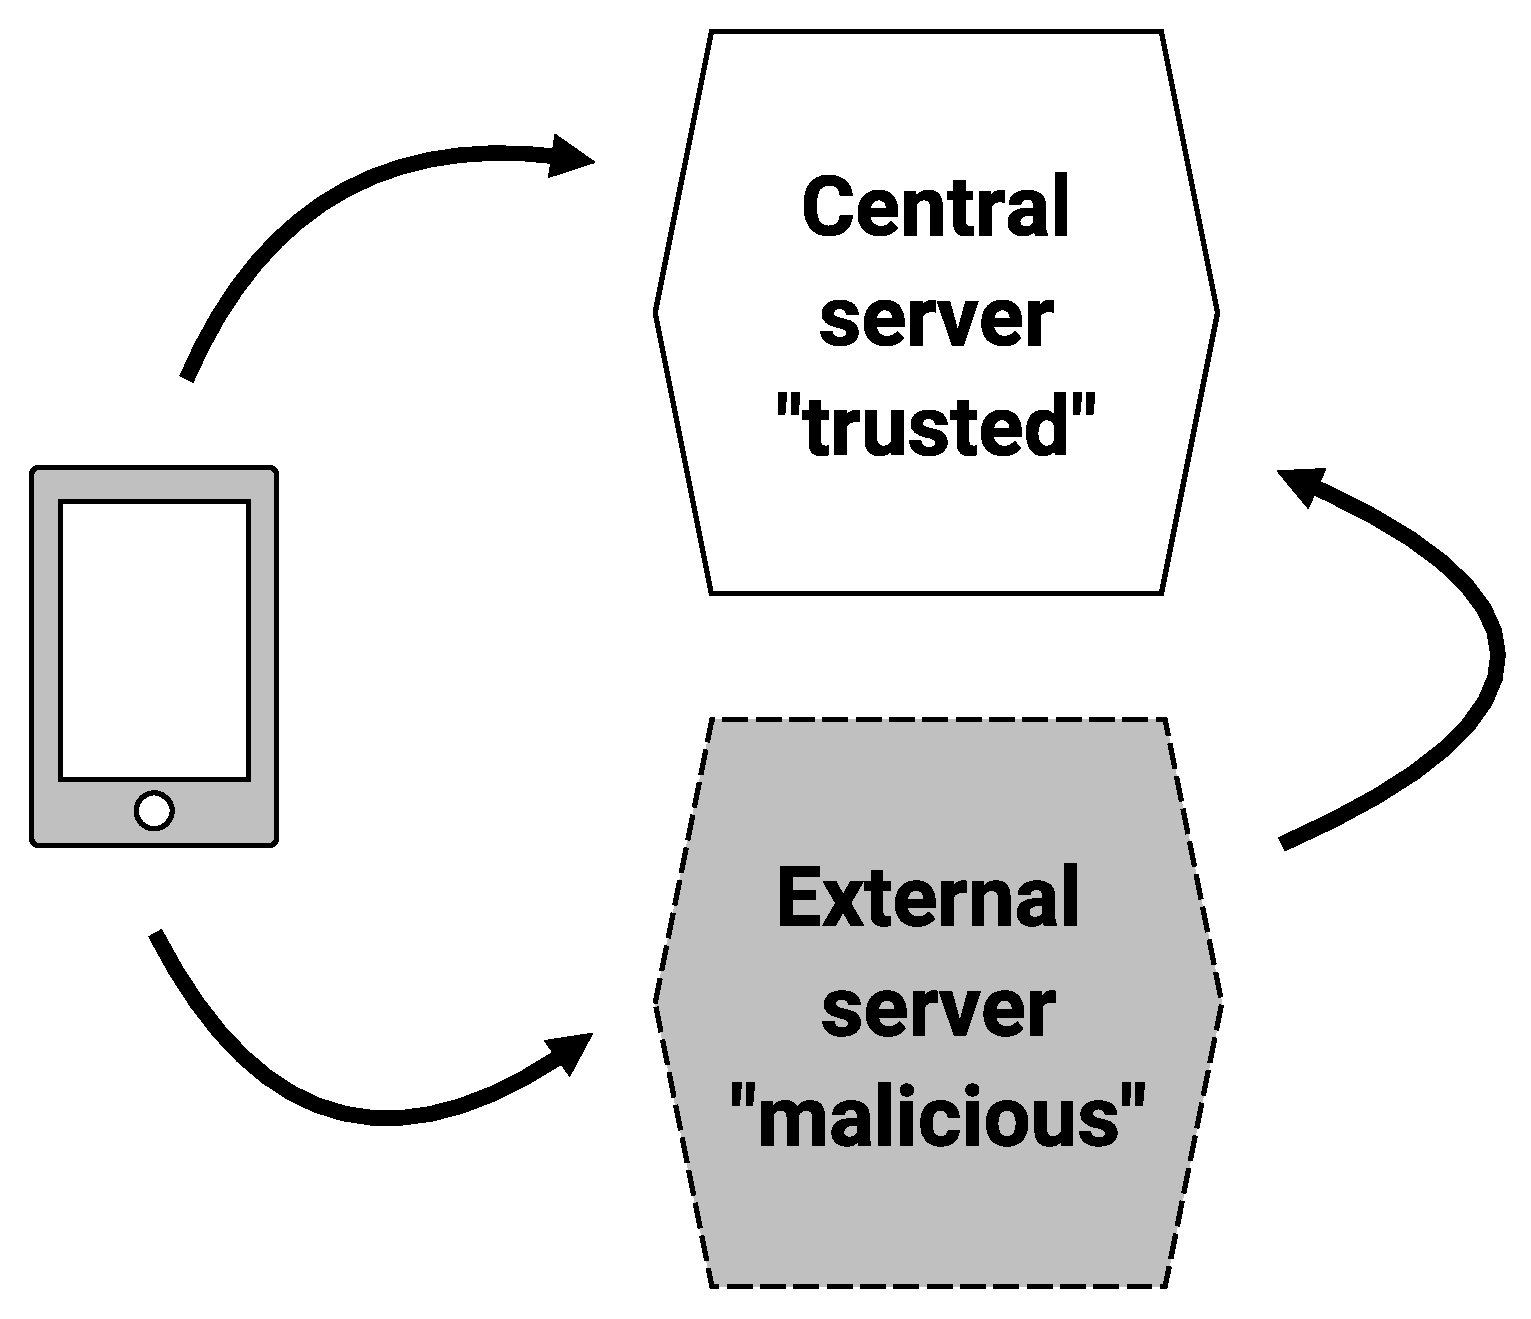
\includegraphics[width=0.4\textwidth]{figures/threat}
    \caption{\label{Threat} APISENSE data collection threat}
\end{figure*}

%%%%%%%%%%%%%%%%%%%%%%%%%%%%%%%%%%%%%%%%%%%%%

Let imagine a user that participate to a data collect campaign.
Currently, the user produces data and sends it directly to a collect server.
The server that collect the data can be the central server or, as exposed before, an external server managed by an organization.

When the user send his data to the central server, the data can directly go to the central server or to an external one.
In this case the server that receive the data knows that the user is iremediably the producer of the data.

Even if we have a strong trust in the central server about keeping users' data safe, this server is a target of choice for an attacker.
The security of the server can be compromized and users data can be stollen in a single attack on the server.
This kind of architecture is not safe because of its single rupture point.

Moreover, in the case of APISENSE architecture, collect servers can be maintain by other organizations that could keep informations about users before sending their data to the trusted central server.
This kind of treats is not acceptable in a privacy way.

To address this scenario, we think-off a method where user is able to send data that he does not produce: data that come from other users.



%%%% OK

\subsection{Goals: Enabling Decentralized Dissemination}

The main goal is to provide a decentralized data dissemination approach that could protect the users' privacy in an untrusted environment.
We want to trend to a solution that could take the advantages of a Privacy by design approach which leads to a minimal intrinsically privacy-preserving system.
Ultimately, our objective is to break the ability of an end-server to link a data to his producer without compromising the quality and the utility of the whole dataset.

%%%% END OK